%  Typ dokumentu - článek, prezentace aj.
\documentclass[english]{article}

%  Nastaví vstupní a výstupní kódování znaků (encoding) a lokalizace
\usepackage[T1]{fontenc}
\usepackage[utf8]{inputenc}
\usepackage[english,czech]{babel}
\usepackage{icomma}

%  Formát papíru a odsazení od jeho okrajů
\usepackage[letterpaper]{geometry}
\geometry{verbose,tmargin=1.5cm,bmargin=2cm,lmargin=2cm,rmargin=2cm}

%  Umožňuje pracovat s grafikou
\usepackage{graphicx}
\usepackage{bigstrut}
\usepackage{epstopdf}

%  Automaticky odsadí i první paragraf v každé sekci
\usepackage{indentfirst}

%  Umožňuje rozdělovat obsah na více sloupců
\usepackage{multicol}
\usepackage{booktabs}
\usepackage{pgffor}

%  Umožňuje používat hypertextové odkazy, nastavuje jejich barvu a
%  vlastnosti
\usepackage[unicode]{hyperref}
\hypersetup{
colorlinks=true, citecolor=blue, filecolor=blue, linkcolor=blue,
urlcolor=blue
}

%  Umožnění odstranění italiky u jednotek
\newcommand{\unit}[1]{\mathrm{#1}}

%  Formátování stránek, empty = odstraní číslování
% \pagestyle{empty}

%  Řádkování
\linespread{1.2}

%  Lepší zobrazování matematiky (rozšíření sum o \limits atd.)
\everymath{\displaystyle}
\usepackage{amsmath, amsthm, amssymb}

% Umožní psát přes \mathbb{N/R/Q/..} množiny čísel
\usepackage{amssymb}

%  Velikost fontu matematických výrazů v dokumentu lze pro danou
% základního fontu dokumentu upravit pomocí:
% \DeclareMathSizes{X}{Y}{Z}{U} kde:
% X je velikost fontu v dokumentu, pro kterou se matematika upraví
% Y je standartní velikost fontu matematiky
% Z je velikost fontu zmenšených (vnořených výrazů)
% U je velikost fontu ještě více zmenšených (vnořených výrazů).
\DeclareMathSizes{10}{10.5}{9}{9}

%  Nastaví autora, název, datum, skupinu měření apod. (můj vlastní
% příkaz, umožní znovu-použití v dokumentu)
\newcommand{\Author}{David Roesel}
\newcommand{\Coauthor}{Tereza Schönfeldová}
\newcommand{\Institute}{FJFI ČVUT v Praze}
\newcommand{\Subject}{FYZIKÁLNÍ PRAKTIKUM II}
\newcommand{\Group}{7}
\newcommand{\Circle}{ZS 7}
\newcommand{\Title}{Úloha \#13b  \\Měření teploty plazmatu v tokamaku GOLEM}
\newcommand{\Date}{17.3.2014}

% Začátek dokumentu - Formátování na výstup
\begin{document}

% Interní proměnné, možno zobrazovat u prezentací, používají se při
% generování pomocí \titlepage apod.
\author{\Author}
\title{\Title}
\date{\Date}

%  Lokalizace některých názvů do češtiny
\renewcommand{\figurename}{Obr.}
\renewcommand{\tablename}{Tab.}
\renewcommand{\refname}{Reference}

% --- Hlavička dokumentu -----------------------------------------------

\setlength{\parindent}{0cm}
\begin{multicols}{2}
\textbf{\Subject \\
        \Institute \\[0.1cm]
%\large  \Title \\[0.5cm]
\Title \\[0.5cm]
}
\begin{tabular}{rlrl}
\large Datum měření: & \Date & \large Skupina: & \Group \\
\large Jméno: & \Author & \large Kroužek:  & \Circle\\
\large Spolupracovala: & \Coauthor &\large Klasifikace:\\
\end{tabular}

\begin{flushright}

\includegraphics[scale=0.28]{../../_meta/fjfi_standart.pdf}
\hspace{0.2cm}

\includegraphics[scale=0.28]{../../_meta/cvut_standart.pdf}
\end{flushright}
\end{multicols}
\hrule
\vspace{0.5cm}

% ----------------------------------------------------------------------


% --- Tělo dokumentu ---------------------------------------------------
\setlength{\parindent}{0.5cm}
\section{Pracovní úkoly}
	  \begin{enumerate}
\item Nalezněte optimální parametry pro nastavení rozmítacího zdroje, aby se proměřovala především iontově nasycená část V-A charakteristiky. Zdůvodněte vámi zvolené parametry.
\item Vykonejte sérii výbojů s různým nastavením parametrů plazmatu. Do protokolu vyneste časovou závislost $U_{fl}$, $\overline{T_{e}}$, $U$ a $I$ pro tři z nich (t.j. 1 graf s 3 křivkami pro $U_{fl}$, 1 takový graf také pro $\overline{T_e}$, atd.)
\item V každém ze tří výbojů předešlého úkolu si vyhlédněte oblast s relativně stálým $U_{fl}$ a $\overline{T_{e}}$. Pro každý výstřel vyneste do grafu V-A charakteristiku přes tyto intervaly. Nafitujte horní část V-A charakteristiky dle vztahu (\ref{eq:fit}) a určete lokální $T_{e}$. Srovnejte s $\overline{T_{e}}$.
\item Zvolte si pevně sadu parametrů výboje a vykonejte další sérii alespoň tří stejných výstřelů. Po každém výstřelu prohoďte rozmítací obvod na sondu na jiné pozici (tj. jiném r). Zvolte si pevně časový interval a určete lokální $T_{e}$ v tomto čase metodou z úkolu 3 pro každý z těchto výbojů.
\item Vztahem (\ref{eq:vztah_teplot}) určete z teplot z předešlého úkolu hloubku sondy v plazmatu. Do protokolu vyneste závislost hloubky určené z teploty na poloze sondy a proložte tuto závislost vztahem $y= Ax+B$. Diskutujte parametry $A$ a $B$.
	  \end{enumerate}

\section{Vypracování}

	\subsection{Použité přístroje}
		Tokamak GOLEM s diagnostikou a datovými sběry, frekvenční generátor, napěťový zesilovač, dělič napětí 1:100, stejnosměrný zdroj 50 V, osciloskop, proměnný odpor, regulační transformátor, 16 Langmuirových sond na vertikálním manipulátoru, programy \emph{GNUplot}, \emph{Enthought Canopy} a \emph{Python}.
					
	\subsection{Teoretický úvod}
		\subsubsection{Plazma}
			Plazma je kvazineutrální (jeho makroskopický náboj je nulový a reaguje jako celek na přítomnost elektromagnetických polí) plyn složený převážně z elektronů a iontů. Vlastnosti plazmatu se, hlavně z důvodu odlišných interakcí, liší od klasického plynu. Jednotlivé části plazmatu spolu v tokamaku interagují prostřednictvím magnetických a elektrických polí o dalekém dosahu (až metry). 
			
			\begin{figure}[h]
			\centering
			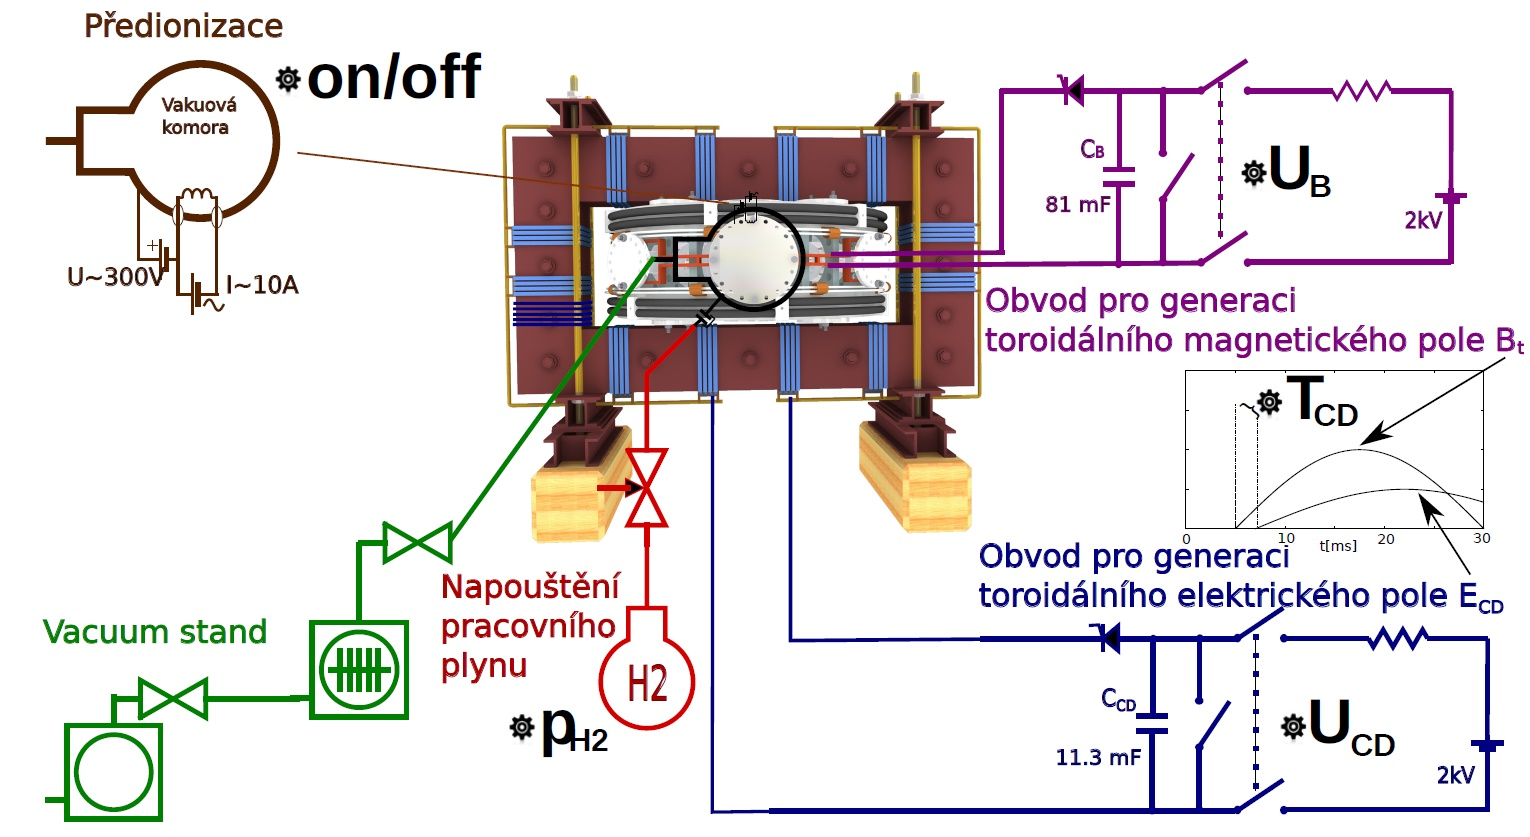
\includegraphics[width=15cm]{att/tokamak.jpg}
			\caption{Schéma tokamaku GOLEM s naznačeným průběhem vybití kondenzátorových baterií a zobrazením nastavitelných parametrů experimentu. Převzato z \cite{bib:zadani}.}
			\label{fig:s_tokamak}
			\end{figure}			
			
			Vysokoteplotní plazma se typicky generuje v zařízení zvaném \emph{tokamak}, jehož zapojení je znázorněno na Obr.~\ref{fig:s_tokamak}. Jedná se o transformátor, který má za svůj jediný sekundární závit právě vysokoteplotní a dobře vodivé plazma. To je uzavřeno ve vakuové nádobě toroidálního tvaru, na kterém je navinuta cívka vytvářející toroidální magnetické pole. 
			
		\subsubsection[Určení Te plazmatu]{Určení $\overline{T_e}$ plazmatu}
			Průměrnou elektronovou teplotu plazmatu $\overline{T_e}$ můžeme vypočítat pomocí vztahu 
			\begin{equation}
				\overline{T_e}~\unit{[eV]}=0,214\left(\frac{Z_{eff} I_p}{U_{loop}}\right)^{2/3},
				\label{eq:vypocet_prumerne_teploty}
			\end{equation}
			kde $Z_{eff}\approx2,5$ je efektivní náboj vodíkového plazmatu, $U_{loop}$ napětí na závit a $I_p$ proud plazmatem.
			
			\begin{figure}[h]
			\centering
			\begin{minipage}[t]{.40\textwidth}
			  \centering
							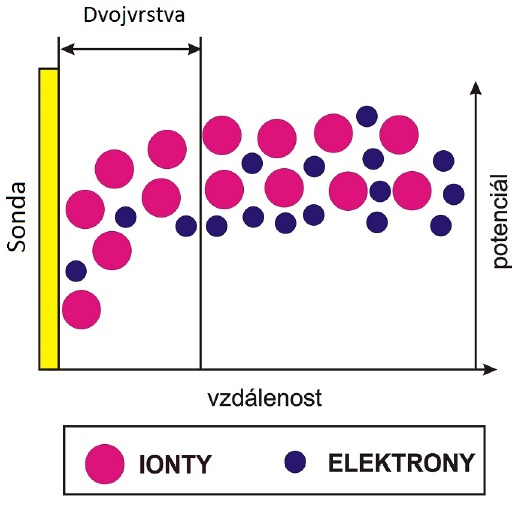
\includegraphics[width=6cm]{att/dvojvrstva.jpg}
							\caption{Elektrická dvojvrstva v okolí plovoucí sondy. Převzato z \cite{bib:zadani}.}
							\label{fig:s_dvojvrstva}
			\end{minipage}%
			\hfill
			\begin{minipage}[t]{.50\textwidth}
			  \centering
							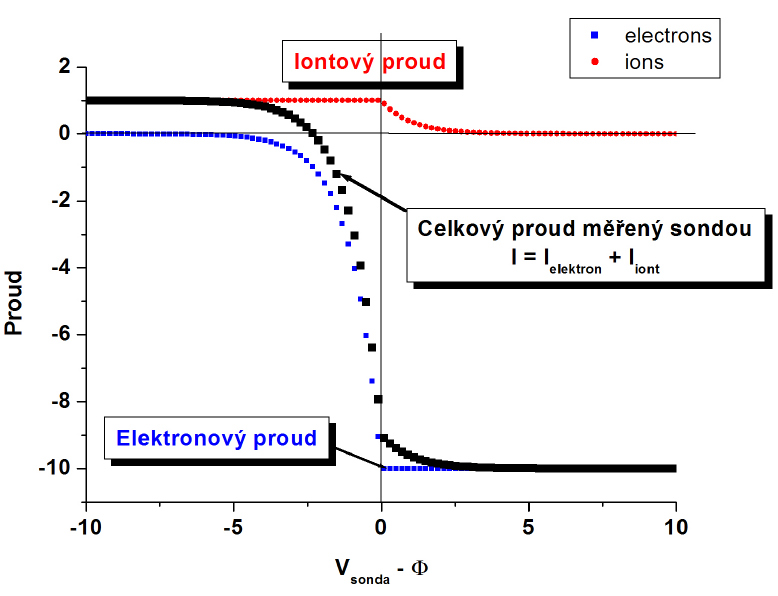
\includegraphics[width=8cm]{att/va.png}
							\caption{Volt-ampérová charakteristika Langmuirovy sondy v plazmatu. Převzato z \cite{bib:zadani}.}
							\label{fig:s_va}
			\end{minipage}
			\end{figure}					
		
		\subsubsection{Sondová měření lokální teploty}
					Pokud není plazma přiliš horké, lze do něj na nějaký čas zasunout takzvanou \emph{Langmuirovu sondu} a měřit pomocí ní lokální $T_e$. Jedná se principem o vodič vnořený do plazmatu, na který dopadají ionty a elektrony. Vzhledem k tomu, že tepelná rychlost je pro elektrony o dva řády vyšší než pro ionty, dopadne jich na nenabitou sondu za určitý čas víc a dojde tak v důsledku k vytvoření takzvané \emph{plazmové dvojvrstvy}, která je znázorněna na Obr.~\ref{fig:s_dvojvrstva}. Díky ní bude v plazmatu vůči zemi (v našem případě komoře) na \emph{plovoucím potenciálu} $U_{fl}$, pro který platí $0 < U_{fl} < \phi$, kde $\phi$ je nenulový potenciál plazmatu.
		
	
		
		\subsubsection[Určení lokální teploty plazmatu]{Určení lokální $T_e$ plazmatu}
			Určení lokální teploty provádíme pomocí tzv. \emph{rake probe}, na které je umístěných 16 Langmuirových sond se vzájemnými vzdálenostmi 2,5 mm. Sonda samotná se nachází 72 mm od středu komory. 
			
			Pro vztah mezi $T_e$ a $\overline{T_e}$ platí
			\begin{equation}
				T_e(r) = 2\overline{T_e}\left(1-\frac{r^2}{a^2}\right) \qquad\rightarrow\qquad r=\sqrt{1-\frac{T_e(r)}{2\overline{T_e}}},
				\label{eq:vztah_teplot}
			\end{equation}
			kde $r$ je poloha sondy v plazmatu a $a=0,085$ m poloměr plazmatu (limiterový). Závislost hloubky určené z teploty na poloze sondy prokládáme lineárním fitem ve tvaru
			\begin{equation}
				y=A\cdot x + B,
				\label{eq:fit_linear}
			\end{equation}				
			kde $A$ udává poměr a $B$ posunutí polohy zjištěné z teploty vůči hloubce sondy. Hodnota $A$ se dá očekávat $A\approx1$, $B$ by se ideálně mělo pohybovat kolem hodnoty $-7,2$ cm jako kompenzace přičtené počáteční poloze.
			
			\begin{figure}[h]
			\centering
			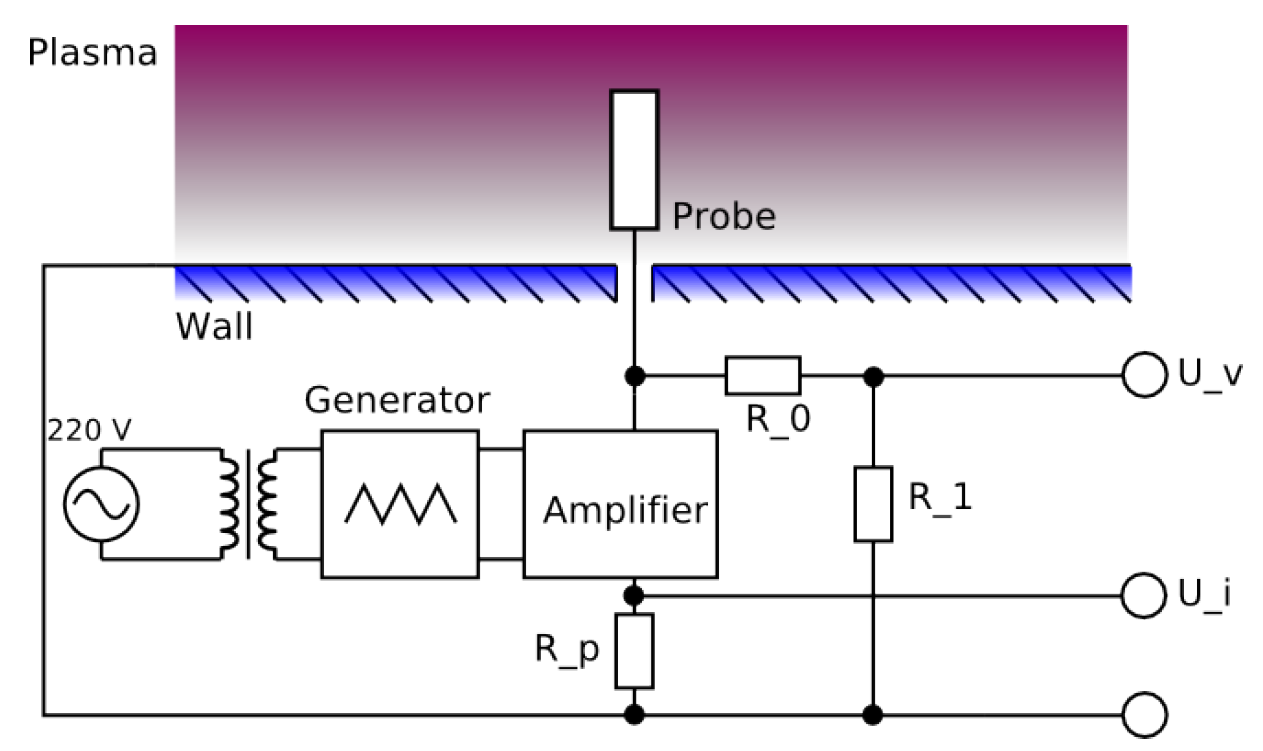
\includegraphics[width=12cm]{att/va_obvod.png}
			\caption{Schéma zapojení obvodu pro rozmítání Langmuirovy sondy k měření její V-A charakteristiky. Převzato z \cite{bib:zadani}.}
			\label{fig:s_va_obvod}
			\end{figure}					
			
			Volt-ampérová charakteristika sondy v plazmatu (viz Obr. \ref{fig:s_va}) je funkcí $T_e$. Při automatizovaně a periodicky prováděné změně $U$ s vysokou frekvencí pomocí frekvenčního generátoru se zpravidla proměřují hodnoty $I$. Schéma zapojení je vidět na Obr. \ref{fig:s_va_obvod}. Napětí na sondě $U$ se měří přes dělič napětí a platí 
			\begin{equation}
					U=100\cdot U_V,
									\label{eq:prepocet_U}
			\end{equation}kde $U_V$ je měřené napětí. Proud ze sondy je měřen přes úbytek napětí $U_I$ na rezistoru o odporu $R_p=22~\Omega$ a platí 
			\begin{equation}
					I=U_I / R_p.
									\label{eq:prepocet_I}
			\end{equation} Z těchto hodnot můžeme sestavit volt-ampérovou charakteristiku, která se pro $U<\phi$ dá popsat vztahem:
			\begin{equation}
				I = I_{i0}\left(1-\unit{exp}\left(e\frac{U-U_{fl}}{kT_e}\right)\right),
			\end{equation}
			kde $U_{fl}$ je výše zmíněný \emph{plovoucí potenciál}, $e$ velikost náboje elektronu, $k$ Boltzmannova konstanta a $I_{i0}$ už iontový nasycený proud. Tento vztah budeme při zpracovávání dat používat ve tvaru
			\begin{equation}
				y=A\left(1-\unit{exp}\left(\frac{x-B}{C}\right)\right),
				\label{eq:fit}
			\end{equation}
			kde $y=I$ [A], $x=U$ [V], $A=I_{i0}$ [A], $B=U_{fl}$ [V] a hledaná $C=T_e$ [eV]. Jako počáteční odhad $T_e$ pro fit používáme $\overline{T_e}$ a $U_{fl}$ s $I_{i0}$ určujeme z naměřených dat. 
			 
	\subsection{Postup měření}
			Nejprve jsme udělali na tokamaku jeden pokusný výstřel, abychom ověřili, že všechno funguje, jak má.  Následně jsme nastavili hodnoty parametrů na frekvenčním generátoru včetně předionizace. Poté jsme provedli další tři výstřely, při kterých jsme různě nastavovali parametry ve webovém rozhraní tokamaku. Z pokusných výstřelu naší a spolupracující skupiny jsme vybrali jeden nejlépe vypadající (\#14681) a čtyřikrát jsme ho zopakovali za prohazování zapojení sond, které měří v tokamaku $T_e$. Námi analyzované výstřely i s parametry jsou vyneseny v Tab. \ref{tab:shotlist}.
			
% Table generated by Excel2LaTeX from sheet 'List1'
\begin{table}[htbp]
  \centering
    \begin{tabular}{|r|r|r|r|r|}
    \hline
    \# výstřelu & $C_{B_t}$ [V] & $C_{CD}$ [V] & $\tau_{CD}$ [ms] & $p_{H_2}$ [mPa] \bigstrut\\
    \hline
    14681 & 900   & 700   & 14    & 13,49 \bigstrut\\
    \hline
    14683 & 900   & 700   & 16    & 11,89 \bigstrut\\
    \hline
    14685 & 700   & 700   & 16    & 11,57 \bigstrut\\
    \hline
    14709 & 900   & 700   & 14    & 12,59 \bigstrut\\
    \hline
    14710 & 900   & 700   & 14    & 13,65 \bigstrut\\
    \hline
    14711 & 900   & 700   & 14    & 13,70 \bigstrut\\
    \hline
    14712 & 900   & 700   & 14    & 13,55 \bigstrut\\
    \hline
    \end{tabular}%
    \caption{Parametry námi analyzovaných výstřelů na tokamaku GOLEM; $C_{B_t}$ je nabití kondenzátoru pro toroidální magnetické pole, $C_{CD}$ nabití kondenzátoru pro toroidální elektrické pole, $\tau_{CD}$ zpoždění elektrického vůči magnetickému poli a $p_{H_2}$ tlak pracovního plynu (vodíku).}
  \label{tab:shotlist}%
\end{table}%
	
	\subsection{Naměřené hodnoty}
			Z webového rozhraní tokamaku jsme získali pět datových souborů pro každý výstřel:
			\begin{itemize}
					\item  \texttt{loop\_voltage\_XXXXX.txt} - obsahující naměřená data pro $U_{loop}$
					\item  \texttt{plasma\_current\_XXXXX.txt} - obsahující naměřená data pro $I_p$		
					\item  \texttt{rake\_probe\_1\_XXXXX.txt} - obsahující naměřená data pro $U_i$, ze kterých získáme podle (\ref{eq:prepocet_I}) proud $I$					
					\item  \texttt{rake\_probe\_2\_XXXXX.txt} - obsahující naměřená data pro $U_{fl}$ - je třeba přepočítat podle (\ref{eq:prepocet_U})
					\item  \texttt{rake\_probe\_3\_XXXXX.txt} - obsahující naměřená data pro $U_v$ - je třeba přepočítat podle (\ref{eq:prepocet_U})										
			\end{itemize}
			Naměřené hodnoty z prvních tří výstřelů pro $U_{fl}$, $U$ a $I$ jsou vyneseny do grafů na Obr.~\ref{fig:g_3Ufl}, \ref{fig:g_3U} a \ref{fig:g_3I}. Závislost průměrné elektronové teploty plazmatu $\overline{T_e}$ každého z nich spočítaná podle (\ref{eq:vypocet_prumerne_teploty}) je vynesena do grafu na Obr.~\ref{fig:g_3Te}. 
			
			Za pomoci takto vynesených závislostí jsme se pokusili určit pro každý výstřel časový interval, na kterém by hodnoty $U_{fl}$ i $\overline{T_e}$ byly co nejkonstantnější a z hodnot $U_v$ a $I$ jsme na takovém časovém intervalu pro každý výstřel sestavili V-A charakteristiku. První třetinu (interval napětí $U$ -100 až -30 V) jejích hodnot na tomto intervalu jsme poté proložili podle (\ref{eq:fit}) a z parametru proložení $C$ jsme určili lokální teplotu plazmatu $T_e$. Pro porovnání jsme na tomto intervalu udělali aritmetický průměr ze spočítaných hodnot $\overline{T_e}$ a získali jsme tak odpovídající údaj i se směrodatnou odchylkou (\ref{eq:smodch_aritmetickeho_prumeru}). Volt-ampérové charakteristiky ve zvolených časových úsecích pro všechny výstřely jsou vyneseny v grafech na Obr.~\ref{fig:g_VA1}, \ref{fig:g_VA2}, \ref{fig:g_VA3}, \ref{fig:g_VA4}, \ref{fig:g_VA5}, \ref{fig:g_VA6} a \ref{fig:g_VA7}. Hodnoty teplot pro jednotlivé výstřely jsou vyneseny v Tab. \ref{tab:teploty}. 
			
% Table generated by Excel2LaTeX from sheet 'List1'
\begin{table}[htbp]
  \centering
    \begin{tabular}{|r|r|r|r|r|}
    \hline
    \# výstřelu & $T_e$ [eV] & $\overline{T_e}$ [eV] & $\Delta t$ [s] & konfigurace sond \bigstrut\\
    \hline
    14681 & $(21,9 \pm 0,5)$ & $( 10,7 \pm  0,1)$ & 0,02250 - 0,02300 & rozmít. \#5, plov. pot. \#4 \bigstrut\\
    \hline
    14683 & $(20,6 \pm 0,5)$ & $( 10,8 \pm  0,1)$ & 0,02475 - 0,02525 & rozmít. \#5, plov. pot. \#4 \bigstrut\\
    \hline
    14685 & $(19,0 \pm 0,6)$ & $( 11,5 \pm  0,1)$ & 0,02445 - 0,02495 & rozmít. \#5, plov. pot. \#4 \bigstrut\\
    \hline
    14709 & $(19,3 \pm 0,8)$ & $( 10,7 \pm  0,1)$ & 0,02250 - 0,02300 & rozmít. \#1, plov. pot. \#2 \bigstrut\\
    \hline
    14710 & $(20,1 \pm 1,1)$ & $( 10,8 \pm  0,1)$ & 0,02250 - 0,02300 & rozmít. \#2, plov. pot. \#1 \bigstrut\\
    \hline
    14711 & $(17,8 \pm 0,5)$ & $( 10,8 \pm  0,1)$ & 0,02250 - 0,02300 & rozmít. \#4, plov. pot. \#5 \bigstrut\\
    \hline
    14712 & $(19,1 \pm 0,4)$ & $( 10,8 \pm  0,1)$ & 0,02250 - 0,02300 & rozmít. \#5, plov. pot. \#4 \bigstrut\\
    \hline
    \end{tabular}%
      \caption{Tabulka naměřených a spočítaných hodnot lokální teploty plazmatu $T_e$ a průměrné elektronové teploty plazmatu $\overline{T_e}$ na časových intervalech $\Delta t$.  }
  \label{tab:teploty}%
\end{table}%
			
			Při posledních čtyřech výstřelech, kterým jsme nechali stejné parametry ve webovém rozhraní, jsme prohazovali rozmítací obvod na sondu na jiné pozici. Za pomoci $T_e$ z fitu V-A charakteristiky a průměrné $\overline{T_e}$ z Tab. \ref{tab:teploty} jsme pak podle (\ref{eq:vztah_teplot}) spočítali hloubku sondy v plazmatu $r$ i s chybou (\ref{eq:chyba_neprime_mereni}) pro každý ze čtyř výstřelů. Takto spočítané hodnoty jsme vynesli do grafu na Obr. \ref{fig:g_hloubka} a proložili podle (\ref{eq:fit_linear}) s výslednými parametry $A=(1,3\pm0,4)$ a $B=(-7\pm3)$~cm. 
			
			Analýza dat byla prováděna pomocí skriptů v jazyce $Python$ v rámci programu $Canopy$. Zdrojové kódy použitých skriptů jsou k dispozici na internetu \cite{bib:repo}.
			
	\subsection{Diskuse}
			\subsubsection{Hledání optimálních parametrů}
					V první části úlohy jsme se snažili najít optimální parametry pro nastavení rozmítacího zdroje, aby se proměřovala především iontově nasycená část volt-ampérové charakteristiky. Na frekvenčním generátoru jsme nastavili režim pily, frekvenci na $\approx4,1$~kHz, amplitudu na $\approx64$~V a DC offset na $\approx-31$~V. Frekvenci bylo třeba nastavit dostatečně vysokou na to, aby za dobu přítomnosti plazmatu stihlo proběhnout alespoň pár V-A charakteristik (půlperiod kmitů). Amplitudu bylo zase třeba nastavit dostatečně vysoko na to, aby se V-A charakteristika dostatečně proměřila. Vzhledem k tomu, že napěťový zesilovač nemá dostatečný výkon pro zvládnutí proudu ze sondy při $U>U_{fl}$, bylo třeba volit záporný DC offset, abychom během rozmítání nepřekračovali plovoucí potenciál.
			
			\subsubsection{Optimalizace parametrů plazmatu}
					Z našich tří úvodních výstřelů se nám nejvíce líbil hned ten první (\#14681), jelikož měl nejkonstantnější úseky ze všech tří. Při tak nízkém počtu zkušebních pokusů ovšem nejde ani zdaleka mluvit o ideálních parametrech a bylo by záhodno udělat výstřelů více. Taktéž by se hodilo mít před vlastním měřením připravené skripty na zpracování dat a moci tak značně urychlit rozpoznávání dobrých a špatných výsledků (např. rychlým výpočtem teploty).
			
			\subsubsection{Voltampérové charakteristiky }
					Dokonale konstantní nebyly $U_{fl}$ ani vypočítaná $\overline{T_e}$ nikdy, i tak se nám však podařilo najít relativně rozumné úseky u každého výstřelu. U průměrné elektronové teploty $\overline{T_e}$ pak vyvstává otázka, jakou chybu u ní brát za správnou. Velikost odchylek hodnot od průměru dosahovala až hodnoty $0,5$~eV, jelikož byl úsek ve většině případů konstantně stoupající, ale standardní chyba aritmetického průměru z dat vycházela kolem $0,01$~eV. Jako kompromis jsme se rozhodli uvádět směrodatnou odchylku (\ref{eq:smodch_aritmetickeho_prumeru}), která podle nás věrohodněji odráží reálnou chybu našich hodnot vzhledem k předpokládanému normálnímu rozdělení.
					
					Nutno podotknout, že se výběrem části dat (podle U) ve V-A charakteristice dají velmi ovlivnit parametry fitu. Pro fit jsme používali jen první zhruba třetinu hodnot (zleva), což je kompromis mezi prokládáním jejich nedostatečného množství a naopak využíváním i méně důvěryhodných hodnot blíže k pravému konci charakteristiky. Reálná chyba lokální teploty $T_e$ bude tedy pravděpodobně větší, než je její fitem určený chybový interval. To, že je $\overline{T_e}$ skoro dvakrát menší než $T_e$ ve většině případech přisuzujeme tomu, že $T_e$ je na rozdíl od $\overline{T_e}$ měřena na jednom konkrétním úseku, takže její hodnota může být odlišná (v našem případě vyšší např. díky poloze úseku blíže středu).
			
			\subsubsection{Závislost hloubky určené z teploty na poloze sondy}
					Námi určené parametry  $A=(1,3\pm0,4)$ a $B=(-7\pm3)$~cm odpovídají (při uvažování chybových intervalů) našim prvotním odhadům. Parametr $A$ určuje, že vypočítaná hloubka sondy odpovídá její reálně poloze, a $B$ může kompenzovat absolutní rozdíl (posunutí) měřené a skutečné vzdálenosti. Oba koeficienty však vyšly se značnou chybou a těžko se z nich tedy usuzuje, jestli naše odhady odpovídají realitě - každopádně je však naše měření nevyloučilo. Výsledky by šlo zpřesnit větším množstvím měření a průměrováním hodnot pro každou z permutací sond. 
						
\section{Závěr}
		Všechna zadaná měření se nám povedla úspěšně provést. Nalezli jsme parametry blízké optimálním pro nastavení rozmítaného zdroje a volbu jsme zdůvodnili.
		
		Vykonali jsme sérii výbojů s různým nastavením parametrů plazmatu a do grafu jsme vynesli časové závislosti $U_{fl}$, $\overline{T_e}$,  $U$ a $I$ pro tři z nich. V každém z těchto výbojů jsme si vyhlédli oblast s relativně stálým $U_{fl}$ a $\overline{T_e}$ a přes tyto intervaly jsme pak do grafu vynesly pro každý výstřel V-A charakteristiku. Její horní část jsme nafitovali pomocí vztahu (\ref{eq:fit}) a určili lokální $T_e$, kterou jsme následně srovnali s $\overline{T_e}$. 
		
		Následně jsme si pevně zvolili sadu parametrů výboje a vykonali jsme další sérii čtyř stejných výstřelů. Po každém výstřelu jsme prohodili rozmítací obvod na sondu na jiné pozici. Pro první tři výstřely jsme si zvolili různé intervaly, pro zbytek výstřelů pak pevně jeden časový interval a určili jsme v nich lokální $T_e$ stejně jako v předchozím úkolu. 
		
		Na závěr jsme vztahem (\ref{eq:vztah_teplot}) určili z předešlého úkolu hloubku sondy v plazmatu. Do grafu jsme vynesli závislost hloubky určené z teploty na poloze sondy a proložili ji vztahem (\ref{eq:fit_linear}), ve kterém jsme diskutovali parametry $A$ a $B$.
	
%\begin{equation}
%	  f(x) =	(0.0121 \pm 0.0003) \left(1-\mathrm{exp}\left(\frac{x-(-56.1\pm 0.2)}{(21.2\pm 0.7)}\right)\right)
%\end{equation}

\section {Použitá literatura}
% --- Literatura a reference -------------------------------------------
\begingroup
\renewcommand{\section}[2]{}

\begin{thebibliography}{9}
\bibitem{bib:zadani} Kolektiv KF, \emph{Návod k úloze: Měření teploty plazmatu v tokamaku GOLEM} [Online], [cit. \today] \newline http://golem.fjfi.cvut.cz/wiki/TrainingCourses/KFpract/14/Probes/uloha13B.pdf

%\bibitem{bib:h3} Petr Chaloupka, \emph{Jak zpracovávat data} [Online], [cit. \today] \newline  https://dl.dropboxusercontent.com/u/11296940/zfm/h3.pdf

%\bibitem{bib:navody} Kolektiv KF, \emph{Návody k přístrojům} [Online], [cit. \today] \newline http://praktikum.fjfi.cvut.cz/documents/chybynav/navody-o.pdf

\bibitem{bib:chyby} Kolektiv KF, \emph{Chyby měření} [Online], [cit. \today] \newline http://praktikum.fjfi.cvut.cz/documents/chybynav/chyby-o.pdf

\foreach \n in {14681, 14683, 14685, 14709, 14710, 14711, 14712}{
\bibitem{bib:shot_\n} GOLEM Team, \emph{Tokamak GOLEM - Shot Database - \n} [Online], [cit. \today] \newline http://golem.fjfi.cvut.cz/shots/\n/
}

%\bibitem{bib:ctverce} Kolektiv KACH UPOL, \emph{Hodnocení analytických výsledků} [Online], [cit. \today] \newline http://ach.upol.cz/ucebnice/hodnoceni7.htm

%\bibitem{bib:tabulky} J. Mikulčák a kol., Matematické, fyzikální a chemické tabulky \& vzorce. Prometheus,
%Praha 2009.\newline
%ISBN 978-80-7196-264-9

\bibitem{bib:repo} Kolektiv autorů, \emph{Repozitář zdrojů k praktiku} [Online], [cit. \today] \newline  http://github.com/roesel/praktika

\end{thebibliography}
\endgroup
% ----------------------------------------------------------------------
\setcounter{equation}{0}
\numberwithin{equation}{section}
%\clearpage
\part{Přílohy}

\section{Domácí příprava}
	Domácí příprava je přiložena k protokolu.
%\clearpage
\section{Statistické zpracování dat}
	Pro statistické zpracování využíváme aritmetického průměru:
	\begin{equation} \label{eq:aritmeticky_prumer}
	\overline{x} = \frac{1}{n}\sum\limits_{i=1}^{n}x_i,
	\end{equation}

	jehož směrodatnou odchylku spočítáme jako 
	\begin{equation} \label{eq:smodch_aritmetickeho_prumeru}
	\sigma_0 = \sqrt{\frac{1}{n} \sum\limits_{i=1}^{n}\left( x_i - \overline{x} \right)^2 },
	\end{equation}
	
	kde $ x_i $ jsou jednotlivé naměřené hodnoty, $ n $ je počet měření, $ \overline{x} $ aritmetický průměr a $ \sigma_0 $ jeho chyba \cite{bib:chyby}.
	
	
%	jehož chybu spočítáme jako 
%	\begin{equation} \label{eq:chyba_aritmetickeho_prumeru}
%	\sigma_0 = \sqrt{\frac{1}{n(n-1)} \sum\limits_{i=1}^{n}\left( x_i - \overline{x} \right)^2 },
%	\end{equation}
%	
%	kde $ x_i $ jsou jednotlivé naměřené hodnoty, $ n $ je počet měření, $ \overline{x} $ aritmetický průměr a $ \sigma_0 $ jeho chyba \cite{bib:chyby}.
%	
Při nepřímém měření počítáme hodnotu s chybou dle následujících vztahů:
	\begin{equation}
	u = f(x, y, z, \ldots),
	\end{equation}
	\begin{displaymath}
	x = (\overline{x} \pm \sigma_x), \qquad
	y = (\overline{y} \pm \sigma_y), \qquad
	z = (\overline{z} \pm \sigma_z), \qquad
	\ldots,
	\end{displaymath}
	
	kde $ u $ je veličina, kterou určujeme nepřímo z měřených veličin $ x, y, z, \ldots $ 
	
	Pak
	\begin{displaymath}
	\overline{u} = f(\overline{x}, \overline{y}, \overline{z}, \ldots),
	\end{displaymath}
	\begin{equation}\label{eq:chyba_neprime_mereni}
	\sigma_u = \sqrt{\left( \frac{\partial f}{\partial x} \right)^2 \sigma^2_x + \left( \frac{\partial f}{\partial y} \right)^2 \sigma^2_y + \left( \frac{\partial f}{\partial z} \right)^2 \sigma^2_z + \ldots},
	\end{equation}
	\begin{displaymath}
	u = (\overline{u} \pm \sigma_ u).
	\end{displaymath}
%%	
%V případě, že máme několik různě přesných měření stejné veličiny, používáme vztah pro vážený průměr:
%	\begin{equation} 
%	\overline{x}=\frac{\sum\limits_{i=1}^{n}p_{i}x_{i}}{\sum\limits_{i=1}^{n}p_{i}},
%	\end{equation}
%	
%	kde $\overline{x}$ je vážený průměr, $x_{i}$ jsou jednotlivá měření a pro $p_{i}$ platí
%	 
%	\begin{equation}
%	p_{i}=\frac{1}{\sigma_{i}^{2}},
%	\end{equation}
%	
%	kde $\sigma_{i}$ jsou jednotlivé chyby daných měření.
%	 
%	Celkovou chybu tedy vypočítáme ze vztahu
%	\begin{equation} \label{eq:vazeny_prumer}
%	\sigma_{0}=\sqrt{\frac{1}{\sum\limits_{i=1}^{n}p_{i}}}.
%	\end{equation}
%
%\subsubsection{Metoda nejmenších čtverců}
%Snažíme-li se metodou nejmenších čtverců proložit data lineární závislostí $Y_i = ax_i+b$, dosazujeme hodnoty $x_i, y_i$ a snažíme se najít parametry $a$ a $b$ tak, aby byl součet všech kvadratických odchylek $\Delta Y_i^2$ minimální. Toho dosáhneme pomocí následujících vzorců \cite{bib:ctverce} :
%\begin{equation}\label{eq:ctverce_a}
%		a = \frac{n\sum\limits_{i=1}^{n}{x_i y_i}  - \sum\limits_{i=1}^{n}{x_i}\sum\limits_{i=1}^{n}{y_i}}{n\sum\limits_{i=1}^{n}{x_i^2}  - \left(\sum\limits_{i=1}^{n}{x_i}\right)^2}, \qquad \qquad
%		\sigma_a = \sqrt{\frac{n\sum\limits_{i=1}^{n}{(y_i - Y_i)^2} }{(n-2)\left(\sum\limits_{i=1}^{n}{x_i^2}  - \left(\sum\limits_{i=1}^{n}{x_i}\right)^2\right)}},
%\end{equation}
%
%\begin{equation}\label{eq:ctverce_b}
%		b = \frac{\sum\limits_{i=1}^{n}{x_i^2} \sum\limits_{i=1}^{n}{y_i}  - \sum\limits_{i=1}^{n}{x_i}\sum\limits_{i=1}^{n}{x_i y_i}}{n\sum\limits_{i=1}^{n}{x_i^2}  - \left(\sum\limits_{i=1}^{n}{x_i}\right)^2}, \qquad \qquad
%		\sigma_b = \sqrt{\frac{\sum\limits_{i=1}^{n}{x_i^2}\sum\limits_{i=1}^{n}{(y_i - Y_i)^2} }{n(n-2)\left(\sum\limits_{i=1}^{n}{x_i^2}  - \left(\sum\limits_{i=1}^{n}{x_i}\right)^2\right)}}.
%\end{equation}
	
\clearpage
\subsection{Tabulky a grafy}
%
	\begin{figure}[h!]
	\begin{center}
	    \vspace*{-1cm}
		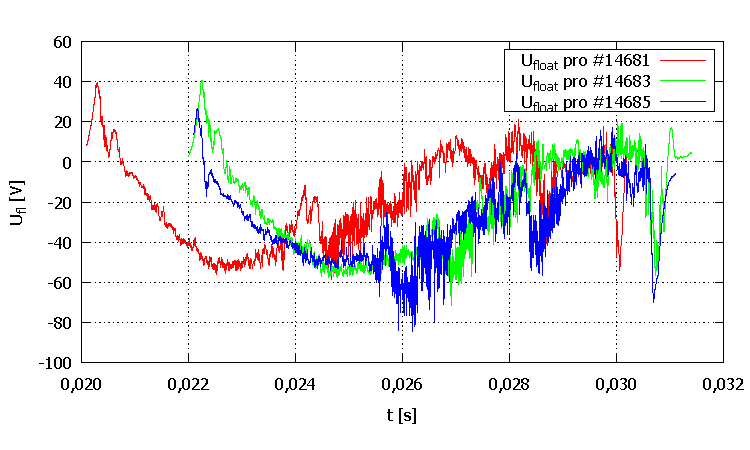
\includegraphics[width=\linewidth]{../gnuplot/135_merge_2.pdf}
	    \vspace*{-1,5cm}
		\caption{Naměřené hodnoty; závislost plovoucího potenciálu $U_{fl}$ na čase $t$ v intervalu existence plazmatu pro první tři výstřely.} 
		\label{fig:g_3Ufl}
	\end{center}
	\end{figure}	
%
	\begin{figure}[h!]
	\begin{center}
	    \vspace*{-1cm}
		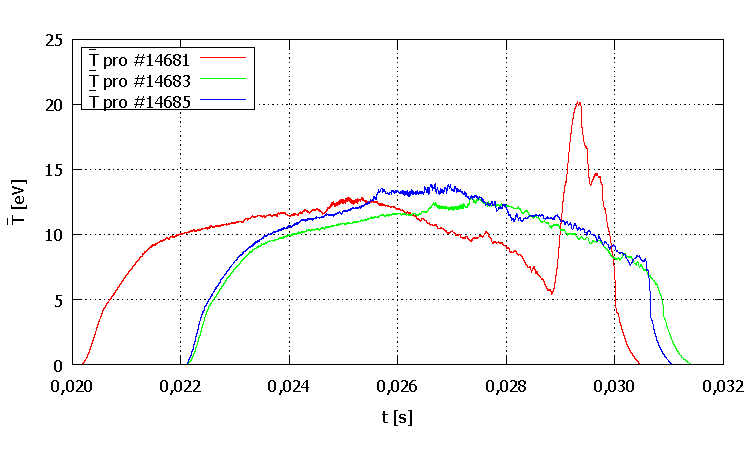
\includegraphics[width=\linewidth]{../gnuplot/135_merge_T.pdf}
	    \vspace*{-1,5cm}
		\caption{Spočítané hodnoty; závislost průměrné elektronové teploty plazmatu $U_{fl}$ na čase $t$ v intervalu existence plazmatu pro první tři výstřely.} 
		\label{fig:g_3Te}
	\end{center}
	\end{figure}	
%
	\begin{figure}[h!]
	\begin{center}
	    \vspace*{-1cm}
		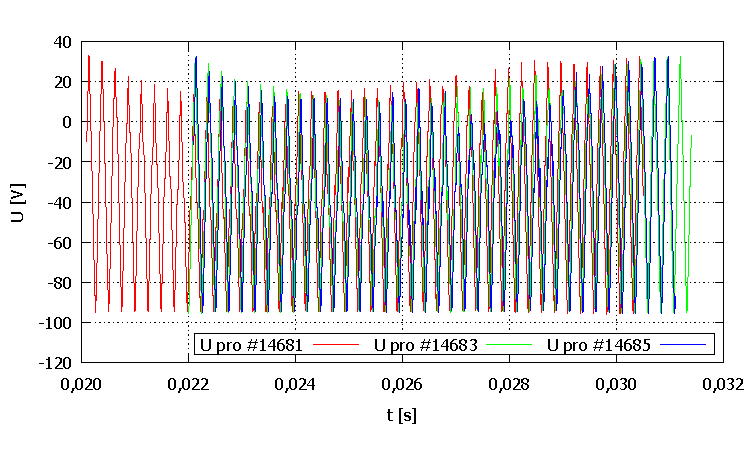
\includegraphics[width=\linewidth]{../gnuplot/135_merge_3.pdf}
	    \vspace*{-1,5cm}
		\caption{Naměřené hodnoty; závislost napětí na sondě $U$ na čase $t$ v intervalu existence plazmatu pro první tři výstřely.} 
		\label{fig:g_3U}
	\end{center}
	\end{figure}
%
	\begin{figure}[h!]
	\begin{center}
	    \vspace*{-1cm}
		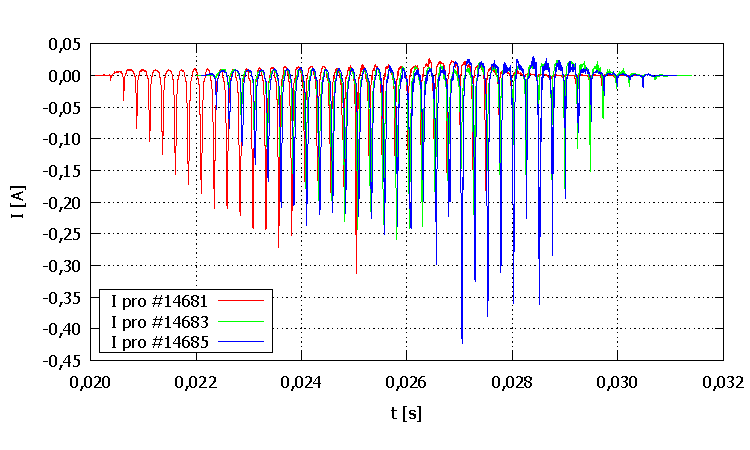
\includegraphics[width=\linewidth]{../gnuplot/135_merge_1.pdf}
	    \vspace*{-1,5cm}
		\caption{Naměřené hodnoty; závislost proudu na sondě $I$ na čase $t$ v intervalu existence plazmatu pro první tři výstřely.} 
		\label{fig:g_3I}
	\end{center}
	\end{figure}
%
	\begin{figure}[h!]
	\begin{center}
	    \vspace*{-1cm}
		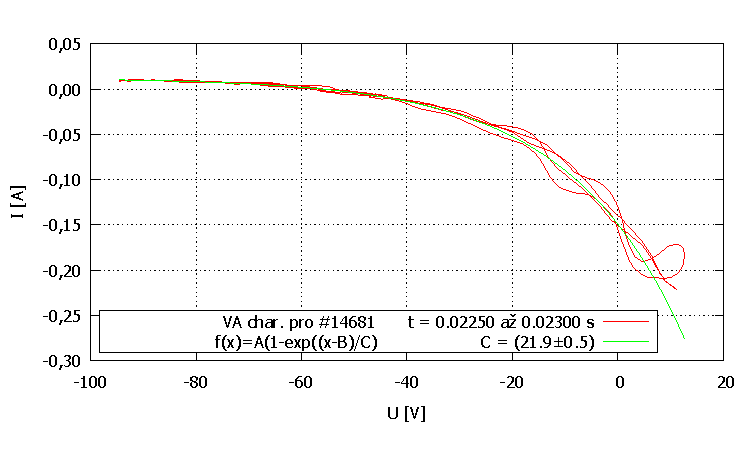
\includegraphics[width=\linewidth]{../gnuplot/VA_merge_14681.pdf}
	    \vspace*{-1,5cm}
		\caption{Volt-ampérová charakteristika výstřelu v příslušném časovém intervalu $t$. } 
		\label{fig:g_VA1}
	\end{center}
	\end{figure}	
%
	\begin{figure}[h!]
	\begin{center}
	    \vspace*{-1cm}
		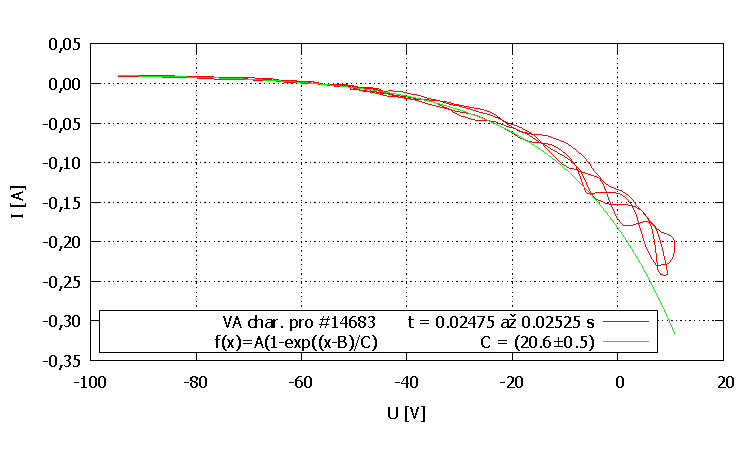
\includegraphics[width=\linewidth]{../gnuplot/VA_merge_14683.pdf}
	    \vspace*{-1,5cm}
		\caption{Volt-ampérová charakteristika výstřelu v příslušném časovém intervalu $t$. } 
		\label{fig:g_VA2}
	\end{center}
	\end{figure}	
%
	\begin{figure}[h!]
	\begin{center}
	    \vspace*{-1cm}
		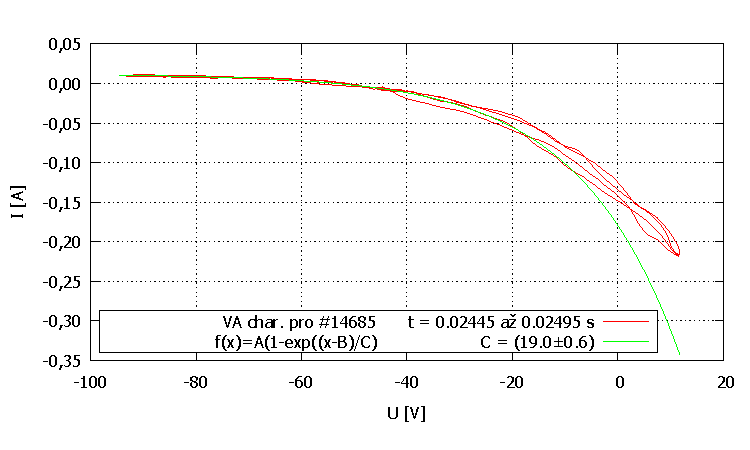
\includegraphics[width=\linewidth]{../gnuplot/VA_merge_14685.pdf}
	    \vspace*{-1,5cm}
		\caption{Volt-ampérová charakteristika výstřelu v příslušném časovém intervalu $t$. } 
		\label{fig:g_VA3}
	\end{center}
	\end{figure}	
%
	\begin{figure}[h!]
	\begin{center}
	    \vspace*{-1cm}
		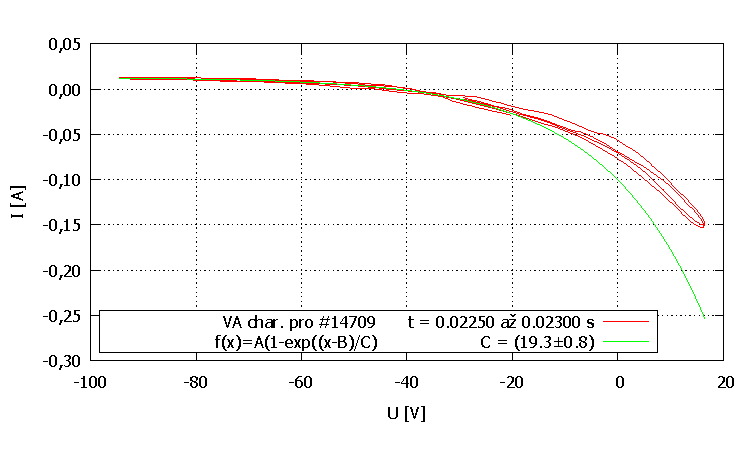
\includegraphics[width=\linewidth]{../gnuplot/VA_merge_14709.pdf}
	    \vspace*{-1,5cm}
		\caption{Volt-ampérová charakteristika výstřelu v příslušném časovém intervalu $t$. } 
		\label{fig:g_VA4}
	\end{center}
	\end{figure}	
%
	\begin{figure}[h!]
	\begin{center}
	    \vspace*{-1cm}
		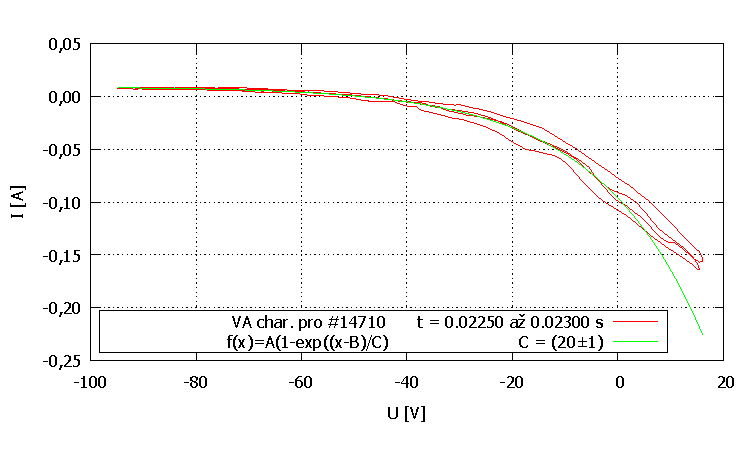
\includegraphics[width=\linewidth]{../gnuplot/VA_merge_14710.pdf}
	    \vspace*{-1,5cm}
		\caption{Volt-ampérová charakteristika výstřelu v příslušném časovém intervalu $t$. } 
		\label{fig:g_VA5}
	\end{center}
	\end{figure}	
%
	\begin{figure}[h!]
	\begin{center}
	    \vspace*{-1cm}
		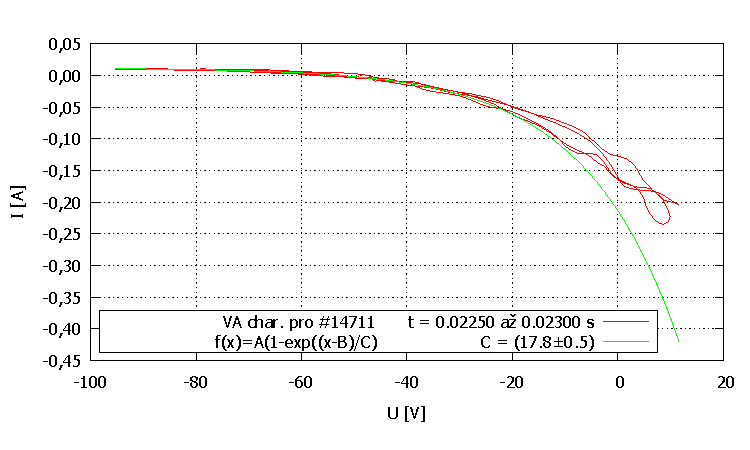
\includegraphics[width=\linewidth]{../gnuplot/VA_merge_14711.pdf}
	    \vspace*{-1,5cm}
		\caption{Volt-ampérová charakteristika výstřelu v příslušném časovém intervalu $t$. } 
		\label{fig:g_VA6}
	\end{center}
	\end{figure}	
%
	\begin{figure}[h!]
	\begin{center}
	    \vspace*{-1cm}
		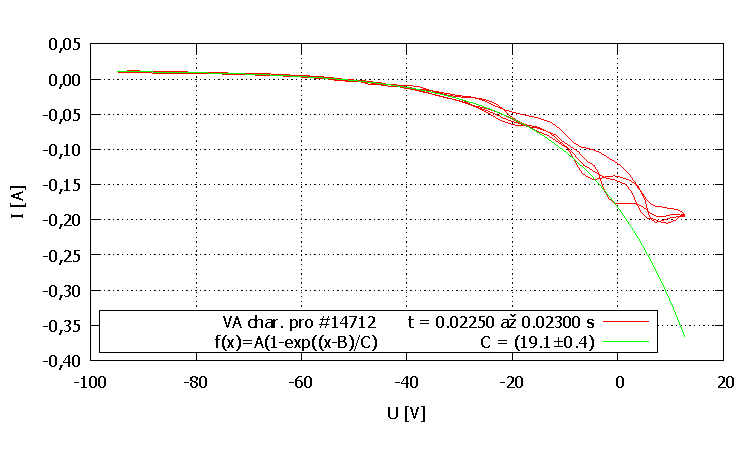
\includegraphics[width=\linewidth]{../gnuplot/VA_merge_14712.pdf}
	    \vspace*{-1,5cm}
		\caption{Volt-ampérová charakteristika výstřelu v příslušném časovém intervalu $t$. } 
		\label{fig:g_VA7}
	\end{center}
	\end{figure}					
%
	\begin{figure}[h!]
	\begin{center}
	    \vspace*{-1cm}
		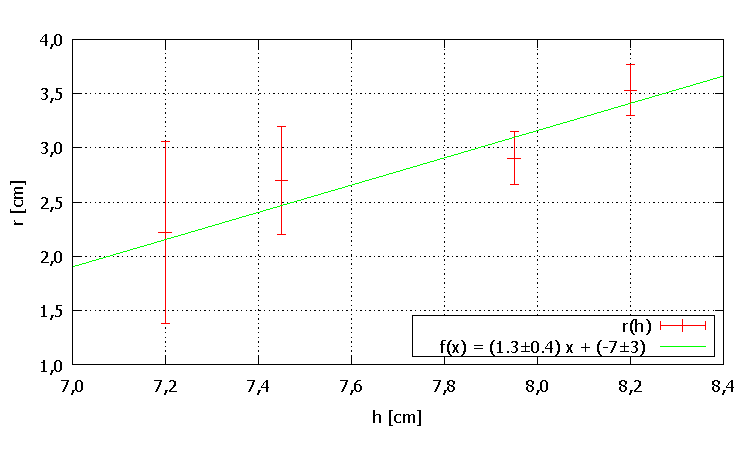
\includegraphics[width=\linewidth]{../gnuplot/r_data.pdf}
	    \vspace*{-1,5cm}
		\caption{Vypočítané hodnoty; závislost polohy sondy $r$ získané z $T_e$ a $\overline{T_e}$ pomocí (\ref{eq:vztah_teplot}) i s chybou (\ref{eq:chyba_neprime_mereni}) na hloubce sondy $h$ pro poslední 4 výstřely. } 
		\label{fig:g_hloubka}
	\end{center}
	\end{figure}					

%\clearpage
%\subsection{Schémata}
%	
%	\begin{figure}[h]
%	\centering
%			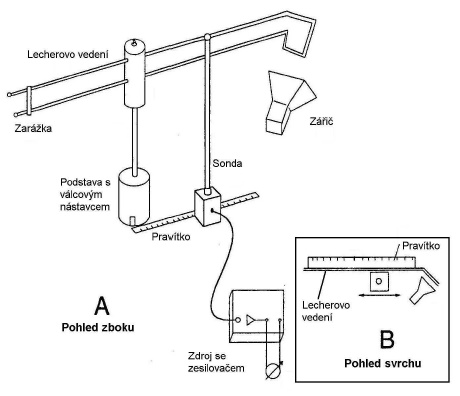
\includegraphics[width=13cm]{att/lecherovo_vedeni.jpg}
%			\caption{Experiment s Lecherovým vedením (převzato z  \cite{bib:zadani}). }
%			\label{fig:lecherovo_vlneni}
%	\end{figure}	
%	
%\clearpage
% --- Konec dokumentu --------------------------------------------------


\end{document}

